\chapter{Implementation}
\label{sec:implementation}
\INITIAL{T}{he proposed method} for implementing an in-situ visualization system is comprised of several vital parts. Although the  output visualization is key from a user perspective, there are important factors to be considered in the way that data is collected and how this method fits into the overarching analysis system. 
 
%%%%%%%%%%%%%%%%%%%%%%%%%%%%%%%%%%%%%%%%%%%%%%%%%%%%%%%%%%%%%%%%%%%%%%%%%%%%
%%%%%%%%%%%%%%%%%%%%%%%%%%%%%%%%%%%%%%%%%%%%%%%%%%%%%%%%%%%%%%%%%%%%%%%%%%%%
\section{Overview}
\label{sec:overview}
\INITIAL{T}{he core development portion of this work} is based on the classes which generate visualizations using a Flink execution plan. Firstly, there is an In-Situ Collector class which has the sole purpose of collecting data sets and/or summaries of data sets as they are run through the Flink analysis task. After data has been collected, the Visualizer can perform various visualization tasks based on the datasets which it has been provided. Figure \ref{fig:uml} shows the basic structural parts of this development. 

\paragraph{Visualization Classes}
While the aforementioned two classes perform the  bulk of the mechanical work, the visualizations themselves each require their own specialized classes which can be invoked generically from the Visualizer. For standard visualizations such as a histogram these classes largely handle the translation of data sets into a more easily digestible format which can be passed to pre-existing classes or visualization libraries. In more complex and specific scenarios such as generating a scatter plot matrix, 'sketches' have been written in the Processing visualization language. These sketches can, with some minor modifications, be used within java projects and then drawn using the java swing toolkit. 

%%%%%%%%%%%%%%%%%%
\begin{figure}
	\centering
	\label{fig:uml}
	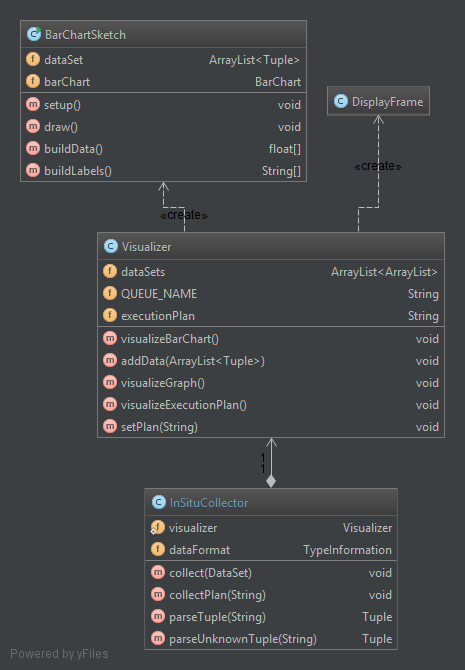
\includegraphics[scale=0.5]{uml_diagram.png}
	\caption{A UML diagram of the core classes}
\end{figure}
%%%%%%%%%%%%%%%%%%

%%%%%%%%%%%%%%%%%%%%%%%%%%%%%%%%%%%%%%%%%%%%%%%%%%%%%%%%%%%%%%%%%%%%%%%%%%%%
%%%%%%%%%%%%%%%%%%%%%%%%%%%%%%%%%%%%%%%%%%%%%%%%%%%%%%%%%%%%%%%%%%%%%%%%%%%%
\section{Data Collection}
\label{sec:data_collection}
\INITIAL{D}{ata types in Flink} are analyzed by the optimizer to determine the most efficient execution strategies. In order to make this process simpler, Flink places limits on the types of data which can be used. There are four categories of types: General objects and POJOs, Tuples, Values, and Hadoop writeables. The handling of each of these types must of course be considered when data is being collected from an analysis graph.

\paragraph{Tuples}
Tuples are used to represent composite data sets, and are composed of a set length list of fields of various types. Tuples can include any valid Flink type as an element, including further tuples. One of the major benefits of using tuple types is the ability to use built-in functions to navigate through the tuple values. Specifically, these functions allow the selection of specific fields as the key for operations and more generally allow the navigation of tuple fields using string expressions.

\paragraph{Data Collector}
The data collector class acts as a simple addition to a pre-existing analysis program in Flink which collects data as it passes through operations. A single collector object exists for a given analysis flow, and collects data at a specific point with a single added line of code calling the collect method. As the data is collected, a user specifies an integer identifier which marks the data set and can be passed to the visualizer later in the task so that the appropriate data set is drawn into whichever visualization is selected. 

\paragraph{Collect Method}
Each time the collect method is called, it sends a new dataset to the central visualizer class. This method accepts a dataset, identifier, and data types as its  arguments and writes this dataset to memory in a format which can be read by the data collector. Each segment of data within a data set object (corresponding to each distributed partition in the overall data flow) is written individually in the same directory of the file system. The writing of this data constitutes a data sink within the execution plan, and thus after each write phase of the data collection process the execute command is called from the analysis program's execution environment. This execution forces the data to be fully recorded before attempts to visualize or collect new data can occur. The data collector then reads this data into a new dataset outside of the original analysis flow's execution environment.

\paragraph{Type Erasure}
Reading the data back into the visualizer after the write operation has occurred is a source of more complication than the collection itself. During the execution of analysis jobs, the compiler will erase types and operate exclusively with generics. This means that when data is extracted from the execution environment for writing and subsequent reading in the collector, the specifics of the original types are not available. For simple data sets, for example exclusively numeric data, it is possible to simply use pattern matching to determine the types of the written data when it is re-read into the collector. However, when handling data sets in which the type is not clear simply from examining a single record this method fails. An simple example of this would be a text data set in which a record consists of a single word; if any numbers such as years or statistics are listed in the text it becomes impossible to determine type from one record alone. Though an issue as simple as this could be avoided through some kind of look ahead sampling method, there is of course also the issue of general data quality. This is particularly unpredictable in the case of in-situ processing. As such, in the collect method the user is required to provide a list of classes which correspond to the respective tuple attributes in the collected set. This allows the collector to assume the type of read data, and eliminates any possible ambiguities. After the read operation occurs, all written data is erased from the file system. 
  
\paragraph{Data Sets}
After data is re-read from the file system by the collector, it is added to the visualizer object. A custom data set class exists for the use of the collector and visualizer. This class is very similar in core function to the data set class which is native to Flink, but allows for the tracking of additional metadata which may be useful for debugging. This information could include timestamps, tags referring to specific operations in the analysis flow, or other semantically relevant information. These datasets are always initialized to contain a list of tuple type objects. As a tuple can of course include any item of a basic type, this implementation will create a tuple of any general object in order to simplify data set operations. For example, if a single integer field is passed through the initial analysis flow, the data set generated in the visualizer will consider this as a tuple of size one which contains an integer.



%%%%%%%%%%%%%%%%%%%%%%%%%%%%%%%%%%%%%%%%%%%%%%%%%%%%%%%%%%%%%%%%%%%%%%%%%%%%
%%%%%%%%%%%%%%%%%%%%%%%%%%%%%%%%%%%%%%%%%%%%%%%%%%%%%%%%%%%%%%%%%%%%%%%%%%%%
\section{Visualization}
\label{visualization}

\INITIAL{D}{eveloping visualizations} in software is a matter of both design and engineering. Finding an effective way to build visuals is often as important as the visualizations themselves. In building the visualizations in this work, different languages and libraries have been applied in order to demonstrate the most important applications of this work in a concise manner. 

\paragraph{Factory Pattern}
The factory pattern is applied in the visualization process, in that a creation method is called from the visualizer at the analysis program level, but a concrete creation method is called from within the visualizer which allows different implementations of the same type of plot to be drawn. This is important for expansion and adaptability of the software, as shifting use-cases and user requirements may require alterations to existing visuals or a complete redesign of some features. This could relate to something as simple as aesthetic changes, such as modifying the way that charts are coloured, to completely redefining the structural elements of charts and their handling of different data types. Additionally, this allows for a combination of custom written classes and libraries to be used if needed so that difficult visualization tasks can be completed.

\paragraph{Processing}
Processing is a language which was initially developed as a teaching tool for computer programming fundamentals which utilized visual arts as a context. It was first released in 2001 as a project of the MIT aesthetics and computation group and has since evolved into a professional level tool for visual programming. The primary advantages of using Processing as a tool for portions of this work are it's ease of use, and compatibility with the rest of the development environment. As it was initially intended as a learning tool, the structure of a processing program is often very simple when compared with something similar generated using only java for example. A single program in Processing is referred to as a "sketch", referring to both the artistic nature of the language and the typical simplicity of it's application. In addition, processing code is compiled into java which simplifies the integration of the two and ensures portability. 

\paragraph{Libraries}
The City University of London's Graphical Information Center provides several useful libraries for performing visualization work. In particular, to aid in the development of work which utilizes processing sketches. The visualizations in this work have been built using utility classes from these libraries in many cases. The libraries provide aesthetic functions for creating charts, such as spacing of axis labels, colouring functions, and bar chart shapes. These functions provide the skeleton for all basic visualizations, upon which logic for handling data and adjusting the specifics of formatting have been added.   

\paragraph{Swing}
Outside of the visualizations themselves, the work of creating frames and navigation is largely handled through directly using java's swing visualization toolkit. A basic JFrame is generated whenever a visualization is created, upon which the visualization is drawn. This frame simply scales to the same size as the visualization it is meant to contain, and acts as an intermediary between the visualizations themselves and the visualizer. 

\paragraph{Visualization Class}
Each visualization class can vary greatly, as their only requirements are that they can be written to a swing panel and that they accept a data set object from the visualizer. All visualizations which have been implemented so far simply consist of setup and draw methods, as well as any utility functions which may be required. The utility functions generally consist of taking the data from the data set and formatting it for consumption into pieces of the visualization such as the axes or bars/lines/etc. In the most complex case,the scatter plot matrix, the visualization class actually divides the data set into segments and generates sub visualizations for each square in the matrix. It is possible for any visualization to rely on a number of utility classes and libraries as long as the top level visualization class still meets the basic requirement of fitting into a single frame. 

\paragraph{Adjusting Visualizations}
The currently implemented visualizations have a certain degree of adaptability built in. For example, axes and overall size of elements will scale based on the data set to be visualized. However, there are some features which are not automatically determined. An example of this would be the use of logarithmic axis scaling. Though it is plausible that a generic enough visualization could be developed for most cases, it is likely that there will always be an edge case based on the usage scenario in which a user will have specific demands of the chart. In such cases, it will be required that the user modify the code in the visualization class itself such that their needs are met. Alternatively, a second modified version of the visualization could be created so that either could be generated alternatively in the same execution of an analysis program. 

\paragraph{Presentation of Visualizations}
PDF collection.
